%iffalse%\let\negmedspace\undefined
\let\negthickspace\undefined
\documentclass[journal,12pt,onecolumn]{IEEEtran}
\usepackage{cite}
\usepackage{amsmath,amssymb,amsfonts,amsthm}
\usepackage{algorithmic}
\usepackage{graphicx}
\usepackage{textcomp}
\usepackage{xcolor}
\usepackage{caption}
\usepackage{txfonts}
\usepackage{listings}
\usepackage{enumitem}
\usepackage{mathtools}
\usepackage{gensymb}
\usepackage{comment}
\usepackage[breaklinks=true]{hyperref}
\usepackage{tkz-euclide} 
\usepackage{listings}
\usepackage{gvv}                                        
%\def\inputGnumericTable{}                                 
\usepackage[latin1]{inputenc}   
\usepackage{xparse}
\usepackage{color}                                            
\usepackage{array}                                            
\usepackage{longtable}                                       
\usepackage{calc}                                             
\usepackage{multirow}
\usepackage{multicol}
\usepackage{hhline}                                           
\usepackage{ifthen}                                           
\usepackage{lscape}
\usepackage{tabularx}
\usepackage{array}
\usepackage{float}
\newtheorem{theorem}{Theorem}[section]
\newtheorem{problem}{Problem}
\newtheorem{proposition}{Proposition}[section]
\newtheorem{lemma}{Lemma}[section]
\newtheorem{corollary}[theorem]{Corollary}
\newtheorem{example}{Example}[section]
\newtheorem{definition}[problem]{Definition}
\newcommand{\BEQA}{\begin{eqnarray}}
\newcommand{\EEQA}{\end{eqnarray}}
\usepackage{float}
%\newcommand{\define}{\stackrel{\triangle}{=}}
\theoremstyle{remark}
\usepackage{ circuitikz }
%\newtheorem{rem}{Remark}
% Marks the beginning of the document this one
\title{ AE : AEROSPACE ENGINEERING}
\author{EE25BTECH11018-Darisy Sreetej}
\begin{document}
\maketitle

\begin{enumerate}
  
\item The function defined by
$
f(x) = \begin{cases}
\sin x, & x < 0 \\
0, & x = 0 \\
3x^3, & x > 0
\end{cases}
$

\begin{enumerate}
\begin{multicols}{2}
\item  is neither continuous nor differentiable at $x = 0$ 
\item  is continuous and differentiable at $x = 0$ 
\item  is differentiable but not continuous at $x = 0$ 
\item  is continuous but not differentiable at $x = 0$
\end{multicols}
\end{enumerate}

\hfill(GATE AE 2008)
\quad

\item The product of the eigenvalues of the matrix
$
\myvec{
1 & 0 & 1 \\
0 & 2 & 1 \\
1 & 1 & -3
}
$
is 
\begin{enumerate}
\begin{multicols}{4}
    

\item 4  \item 0  \item $-6$  \item $-9$
\end{multicols}
\end{enumerate}
\hfill(GATE AE-2008)
\quad

\item Which of the following equations is a LINEAR ordinary differential equation?

\begin{enumerate}
\begin{multicols}{2}
   \item $\dfrac{d^2 y}{dx^2} + \dfrac{dy}{dx} + 2y^2 = 0$
    \item $\dfrac{d^2 y}{dx^2} + y \dfrac{dy}{dx} + 2y = 0$
    \item $\dfrac{d^2 y}{dx^2} + \dfrac{dy}{dx} + 2y = 0$
   \item $\left( \dfrac{dy}{dx} \right)^2 + \dfrac{dy}{dx} + 2y = 0$
   \end{multicols}
\end{enumerate}
\hfill(GATE AE-2008)
\quad

\item To transfer a satellite from an elliptical orbit to a circular orbit having radius equal to the apogee distance of the elliptical orbit, the speed of the satellite should be 
\begin{enumerate}
    \begin{multicols}{2}

\item increased at the apogee 
\item decreased at the apogee 
\item increased at the perigee 
\item decreased at the perigee
\end{multicols}
\end{enumerate}
\hfill(GATE AE-2008)
\quad

\item The service ceiling of a transport aircraft is defined as the altitude 
\begin{enumerate}
    \begin{multicols}{2}
\item that is halfway between sea-level and absolute ceiling 
\item at which it can cruise with one engine operational 
\item at which its maximum rate of climb is zero 
\item at which its maximum rate of climb is 0.508 m/s
\end{multicols}
\end{enumerate}

\hfill(GATE AE-2008)
\quad

\item The drag of an aircraft in steady climbing fight at a given forward speed is 
\begin{enumerate}
\begin{multicols}{2}
    \item inversely proportional to climb angle 
    \item higher than drag in steady level fight at the same forward speed 
    \item lower than drag in steady level fight at the same forward speed 
    \item independent of climb angle 
    \end{multicols}
\end{enumerate}
\hfill(GATE AE-2008)

\quad

\item In steady,level turning flight of an aircraft at a load factor 'n',the ratio of the horizontal component of lift and aircraft weight is 
\begin{enumerate}
\begin{multicols}{4}
    \item $ \sqrt{n-1} $
    \item $\sqrt{n+1}$
    \item $\sqrt{n^2-1}$
    \item $\sqrt{n^2+1}$
    \end{multicols}
\end{enumerate}
\hfill(GATE AE-2008)

\quad

\item The parameters that remain constant in a cruise-climb of an aircraft are
\begin{enumerate}
\begin{multicols}{2}
    \item equivalent airspace and lift coefficient 
    \item altitude and lift coefficient
    \item equivalent airspace and altitude 
    \item lift coefficient and aircraft mass 
    \end{multicols}
\end{enumerate}
\hfill(GATE AE-2008)

\quad

\item The maximum thickness to chord ratio for the NACA 24012 airfoil is  
\begin{enumerate}
\begin{multicols}{4}
    \item 0.01 
    \item 0.12
    \item 0.24 
    \item 0.40
    \end{multicols}
\end{enumerate}
\hfill(GATE AE-2008)

\quad

\item The maximum possible value of pressure coefficient \(C_p\) in incompressible flow is 
\begin{enumerate}
\begin{multicols}{4}
    \item 0.5
    \item 1 
    \item $pi$
    \item $infty$
    \end{multicols}
\end{enumerate}
\hfill(GATE AE-2008)

\quad

\item An irrotational and inviscid flow can become rotational on passing through a 
\begin{enumerate}
\begin{multicols}{2}
    \item normal shock wave 
    \item oblique shock wave 
    \item curved shock wave 
    \item mach wave 
    \end{multicols}
\end{enumerate}
\hfill(GATE AE-2008)

\quad 

\item Laminar flow airfoils are used to reduce 
\begin{enumerate}
\begin{multicols}{2}
    \item trim drag 
    \item skin friction drag 
    \item induced drag 
    \item wave drag
    \end{multicols}
\end{enumerate}
\hfill(GATE AE-2008)

\quad 

\item The degree of reaction of an impulse turbine is 
\begin{enumerate}
\begin{multicols}{4}
    \item 1
    \item 0.75 
    \item 0.5
    \item 0
    \end{multicols}
\end{enumerate}
\hfill(GATE AE-2008)

\quad 

\item In a convergent-divergent(CD) nozzle of a rocket motor, the wall heat flux is maximum at 
\begin{enumerate}
\begin{multicols}{2}
    \item the exit of the divergent portion of the CD nozzle 
    \item the entry to the convergent portion of the CD nozzle 
    \item the throat of the CD nozzle 
    \item the mid-length of the divergent portion of the CD nozzle 
    \end{multicols}
\end{enumerate}
\hfill(GATE AE-2008)

\quad 

\item In a scramjet engine, the Mach number at the entry to the combustion chamber is around 
\begin{enumerate}
\begin{multicols}{4}
    \item 0
    \item 0.3
    \item 2
    \item 6 
    \end{multicols}
\end{enumerate}
\hfill(GATE AE-2008)

\quad 

\item DB denotes double base solid propellant.  
LOX-RP1 denotes liquid oxygen -- kerosene combination.  
LOX-LH$_2$ denotes liquid oxygen -- hydrogen combination.  

The correct order of increasing specific impulse is:  

\begin{enumerate}
\begin{multicols}{2}
\item $\text{DB} < \text{LOX-RP1} < \text{LOX-LH}_2$
\item $\text{LOX-RP1} < \text{DB} < \text{LOX-LH}_2$
\item $\text{LOX-LH}_2 < \text{DB} < \text{LOX-RP1}$
\item $\text{DB} < \text{LOX-LH}_2 < \text{LOX-RP1}$
\end{multicols}
\end{enumerate} 
\hfill(GATE AE-2008)

\quad 

\item  In the absence of body moments, the symmetry of the stress of the stress tensor is derived from 
\begin{enumerate}
\begin{multicols}{2}
    \item force equilibrium conditions 
    \item moment equilibrium conditions 
    \item linear relations between stresses and strains 
    \item compatibility conditions 
    \end{multicols}
\end{enumerate}
\hfill(GATE AE-2008)

\quad 

\item  In a 3-D orthotropic material, the number of elastic constants in linear stress-strain relationship is
    
    \begin{enumerate}
    \begin{multicols}{4}
        \item 3
        \item 5
        \item 9
        \item 21
        \end{multicols}
    \end{enumerate}
\hfill(GATE AE-2008)

\quad

    \item The compatibility conditions in theory of elasticity ensure that
    \begin{enumerate}
    \begin{multicols}{2}
        \item there is compatibility between various direct and shear stresses
        \item relationships between stresses and strains are consistent with constitutive relations
        \item displacements are single-valued and continuous
        \item stresses satisfy bi-harmonic equation
        \end{multicols}
    \end{enumerate}
\hfill(GATE AE-2008)

\quad

    \item In a spring-mass-damper single degree of freedom system, the mass is 2 kg and the undamped natural frequency is 20 Hz. The critical damping constant of the system is
    \begin{enumerate}
        \begin{multicols}{4}
        \item 160$\pi$ Ns/m
        \item 80$\pi$ Ns/m
        \item 1 Ns/m
        \item 0 Ns/m
        \end{multicols}
    \end{enumerate}
\hfill(GATE AE-2008)

\quad


\quad 

        \item Which of the following quantities remains constant for a satellite in an elliptical orbit around the earth?
    \begin{enumerate}
    \begin{multicols}{2}
        \item Kinetic energy
        \item Product of speed and radial distance from the center of the earth
        \item Rate of area swept by the radial vector from the center of the orbit
        \item Rate of area swept by the radial vector from the center of the earth
        \end{multicols}
    \end{enumerate}
\hfill(GATE AE-2008)

    \quad
    
    \item A planet is observed to be at its slowest when it is at a distance $r_1$ from the sun and at its fastest when it is at a distance $r_2$ from the sun. The eccentricity $e$ of the planet's orbit is given by
    \begin{enumerate}
    \begin{multicols}{2}
        \item $e = \frac{r_1}{r_2}$
        \item $e = \frac{r_1 - r_2}{r_1 + r_2}$
        \item $e = \frac{r_2}{r_1}$
        \item $e = \frac{r_1 + r_2}{r_1 - r_2}$
        \end{multicols}
    \end{enumerate}
    \hfill(GATE AE-2008)

\quad

    \item The function $f(x,y,z) = \frac{1}{2}x^2y^2z^2$ satisfies
    \begin{enumerate}
    \begin{multicols}{2}
        \item grad $f = 0$
        \item div(grad $f$) = 0
        \item curl(grad $f$) = 0
        \item grad(div(grad $f$)) = 0
        \end{multicols}
    \end{enumerate}
    \hfill(GATE AE-2008)

    \quad
    
    \item Which of the following is true for all choices of vectors $\vec{p}, \vec{q}, \vec{r}$?
    \begin{enumerate}
    \begin{multicols}{2}
        \item $\vec{p} \times \vec{q} + \vec{q} \times \vec{r} + \vec{r} \times \vec{p} = 0$
        \item $(\vec{p} \cdot \vec{q}) \vec{r} + (\vec{q} \cdot \vec{r}) \vec{p} + (\vec{r} \cdot \vec{p}) \vec{q} = 0$
        \item $\vec{p} \cdot (\vec{q} \times \vec{r}) + \vec{q} \cdot (\vec{r} \times \vec{p}) + \vec{r} \cdot (\vec{p} \times \vec{q}) = 0$
        \item $\vec{p} \times (\vec{q} \times \vec{r}) + \vec{q} \times (\vec{r} \times \vec{p}) + \vec{r} \times (\vec{p} \times \vec{q}) = 0$
        \end{multicols}
    \end{enumerate}
    \hfill(GATE AE-2008)

\quad

    \item  The value of the line integral
    $
    \frac{1}{2\pi} \oint (x\,dy - y\,dx)
    $
    taken anticlockwise along a circle of unit radius is
    \begin{enumerate}
    \begin{multicols}{4}
        \item 0.5
        \item 1
        \item 2
        \item $\pi$
        \end{multicols}
    \end{enumerate}
\hfill(GATE AE-2008)

\quad

    \item Which of the following is a solution of 
    $
    \frac{d^2 y}{dx^2} + 2\frac{dy}{dx} + y = 0 ?
    $
    \begin{enumerate}
    \begin{multicols}{2}
        \item $e^{-x} + xe^{-x}$
        \item $e^x + xe^{-x}$
        \item $e^t + e^x$
        \item $e^{-x} + xe^x$
        \end{multicols}
    \end{enumerate}
    \hfill(GATE AE-2008)

    \quad

    \item Suppose the non-constant functions $F(x)$ and $G(t)$ satisfy
    $
    \frac{d^2 F}{dx^2} + p^2 F = 0,\quad \frac{dG}{dt} + c^2 p^2 G = 0,
    $
    where $p$ and $c$ are constants. Then the function $u(x,t) = F(x)G(t)$ definitely satisfies
    \begin{enumerate}
    \begin{multicols}{2}
        \item $\frac{\partial^2 u}{\partial t^2} = c^2 \frac{\partial^2 u}{\partial x^2}$
        \item $\frac{\partial u}{\partial t} = c^2 \frac{\partial^2 u}{\partial x^2}$
        \item $\nabla^2 u = 0$
        \item $\frac{\partial^2 u}{\partial t^2} + c^2 u^2 = 0$
        \end{multicols}
    \end{enumerate}
    \hfill(GATE AE-2008)

    \quad

        \item The following set of equations
    $
    \myvec{
    1 & 1 & 2 \\
    1 & 0 & 1 \\
    0 & 1 & 1 
    }
    \myvec{
    x_1 \\
    x_2 \\
    x_3
    }
    =
    \myvec{
    1 \\
    -1 \\
    0
    }
    $
    has
    \begin{enumerate}
    \begin{multicols}{2}
        \item no solution
        \item a unique solution
        \item two solutions
        \item infinite solutions
        \end{multicols}
    \end{enumerate}
    \hfill(GATE AE-2008)

    \quad

    \item The function $f(x) = x^2 - 5x + 6$
    \begin{enumerate}
    \begin{multicols}{2}
        \item has its maximum value at $x = 2.0$
        \item has its maximum value at $x = 2.5$
        \item is increasing on the interval (2.0, 2.5)
        \item is increasing on the interval (2.5, 3.0)
        \end{multicols}
    \end{enumerate}
    \hfill(GATE AE-2008)

    \quad

        \item Let $Y(s)$ denote the Laplace transform $\mathcal{L}(y(t))$ of the function $y(t) = \cosh(at) \sin(at)$. Then
    \begin{enumerate}
    \begin{multicols}{2}
        \item $\mathcal{L}\left(\frac{dy}{dt}\right) = \frac{dY}{ds}, \quad \mathcal{L}(t\,y(t)) = sY(s)$
        \item $\mathcal{L}\left(\frac{dy}{dt}\right) = sY(s), \quad \mathcal{L}(t\,y(t)) = -\frac{dY}{ds}$
        \item $\mathcal{L}\left(\frac{dy}{dt}\right) = \frac{dY}{ds}, \quad \mathcal{L}(t\,y(t)) = Y(s-1)$
        \item $\mathcal{L}\left(\frac{dy}{dt}\right) = sY(s), \quad \mathcal{L}(t\,y(t)) = e^{a}Y(s)$
        \end{multicols}
    \end{enumerate}
        \hfill(GATE AE-2008)

    \quad

    \item  The velocity required for a spacecraft to escape earth's gravitational field depends on
    \begin{enumerate}
    \begin{multicols}{2}
        \item the mass of the spacecraft
        \item the distance between earth's center and the spacecraft
        \item the earth's rotational speed about its own axis
        \item the earth's orbital speed
        \end{multicols}
    \end{enumerate}
    \hfill(GATE AE-2008)

    \quad

\item The figure below shows the variation of $C_m$ versus $\alpha$ for an aircraft for three combinations of elevator deflections and locations of centre of gravity.In the figure, lines P and Q are parallel, while lines Q and R have the same intercept on the $C_m$ axis.

\begin{figure}
    \centering
    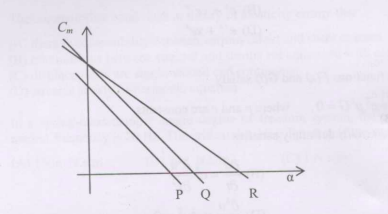
\includegraphics[width=0.5\linewidth]{figs/Screenshot from 2025-08-08 00-10-35.png}
    \caption{Caption}
    \label{fig:placeholder}
\end{figure}
 Which of the following statements is true?
    \begin{enumerate}
    \begin{multicols}{2}
        \item Lines P and Q correspond to the same centre of gravity location.
        \item Lines Q and R correspond to the same centre of gravity location.
        \item Lines P and Q correspond to the same elevator deflection.
        \item Lines P and R correspond to the same centre of gravity location.
        \end{multicols}
    \end{enumerate}
    \hfill(GATE AE-2008)

    \quad

 \item Which of the following statements is TRUE as the altitude increases in stratosphere of International Standard Atmosphere?
    \begin{enumerate}
    \begin{multicols}{2}
        \item Temperature increases and dynamic viscosity decreases.
        \item Temperature remains constant and pressure increases.
        \item Temperature decreases and sound speed decreases.
        \item Temperature remains constant and density decreases.
        \end{multicols}
    \end{enumerate}
    \hfill(GATE AE-2008)

    \quad

 \item Which of the following statements is TRUE?
    \begin{enumerate}
    \begin{multicols}{2}
        \item Wing dihedral reduces roll stability while a low wing increases roll stability.
        \item Wing dihedral increases roll stability while a low wing reduces roll stability.
        \item Wing dihedral, as well as low wing reduces roll stability.
        \item Wing dihedral, as well as low wing increases roll stability.
        \end{multicols}
    \end{enumerate}
    \hfill(GATE AE-2008)

    \quad

 \item An aircraft has a level flight stalling speed of 60 m/s EAS (equivalent air speed). As per the V-n diagram, what is the minimum speed at which it should be designed to withstand the maximum vertical load factor of 9?
    \begin{enumerate}
    \begin{multicols}{4}
        \item 20 m/s
        \item 60 m/s
        \item 120 m/s
        \item 180 m/s
        \end{multicols}
    \end{enumerate}
    \hfill(GATE AE-2008)

    \quad

    \item  Match each mode of aircraft motion listed in Group I to its corresponding property from Group II.

\begin{center}
\begin{tabular}{ll}
    \textbf{Group I} & \textbf{Group II} \\
    P. Ferrite & 1. Hexagonal Close Packed (HCP) \\
    Q. Austenite & 2. Body Centered Cubic (BCC) \\
    R. Martensite & 3. Body Centered Tetragonal (BCT) \\
    & 4. Face Centered Cubic (FCC)
\end{tabular}
\end{center}
    \begin{enumerate}
    \begin{multicols}{2}
        \item P-2, Q-1, R-4, S-3
        \item P-4, Q-3, R-2, S-1
        \item P-4, Q-1, R-2, S-3
        \item P-2, Q-3, R-4, S-1
        \end{multicols}
    \end{enumerate}
    \hfill(GATE AE-2008)

    \quad

    \item An aircraft is cruising at a true air speed (TAS) of 100 m/s under ISA conditions, at an altitude at which the density of free stream is 0.526 kg/m$^3$. What will be the equivalent air speed (EAS)?
    \begin{enumerate}
    \begin{multicols}{2}
        \item 65.5 m/s
        \item 72.5 m/s
        \item 110.5 m/s
        \item 152.7 m/s
        \end{multicols}
    \end{enumerate}
    \hfill(GATE AE-2008)

    \quad

\item In the definition of the aircraft Euler angles $\phi$ (roll), $\theta$ (pitch), and $\psi$ (yaw), the correct sequence of rotations required to make the inertial frame coincide with the aircraft body frame is  
\begin{enumerate}
\begin{multicols}{2}
    \item First $\psi$ about $z$ axis, second $\theta$ about $y$ axis, third $\phi$ about $x$ axis
    \item First $\theta$ about $y$ axis, second $\phi$ about $x$ axis, third $\psi$ about $z$ axis
    \item First $\phi$ about $x$ axis, second $\theta$ about $y$ axis, third $\psi$ about $z$ axis
    \item First $\psi$ about $z$ axis, second $\phi$ about $x$ axis, third $\theta$ about $y$ axis
    \end{multicols}
\end{enumerate}
    \hfill(GATE AE-2008)

    \quad

\item To maximize range of a jet engine aircraft, it should be flown at a velocity that maximizes  
\begin{enumerate}
\begin{multicols}{2}
    \item $C_L/C_D$
    \item $C_L^{0.5}/C_D$
    \item $C_L^{1.5}/C_D$
    \item $C_L^2/C_D$
    \end{multicols}
\end{enumerate}
    \hfill(GATE AE-2008)

    \quad

\item The primary function of the fin in the vertical tail of an aircraft is to provide  
\begin{enumerate}
\begin{multicols}{2}
    \item yaw control
    \item yaw stability
    \item roll damping
    \item roll stability
    \end{multicols}
\end{enumerate}
    \hfill(GATE AE-2008)

    \quad

\item An aircraft requires the trailing edge of the elevator to be deflected upwards from its initial position to lower the trim speed. Which of the following statements about the static stick-fixed stability of this aircraft is true? 
\begin{enumerate}
\begin{multicols}{2}
    \item The aircraft is unstable.
    \item The aircraft is neutrally stable.
    \item The aircraft is stable.
    \item The stability of the aircraft cannot be determined from the given information.
    \end{multicols}
\end{enumerate}
    \hfill(GATE AE-2008)

    \quad

\item Which of the following statements is true for an aircraft flying at a low angle of attack?  
\begin{enumerate}
\begin{multicols}{2}
    \item Yawing motion generates yawing moment and pitching moment.
    \item Rolling motion generates rolling moment and pitching moment.
    \item Yawing motion generates yawing moment and rolling moment.
    \item Pitching motion generates yawing moment and rolling moment.
    \end{multicols}
\end{enumerate}
    \hfill(GATE AE-2008)

    \quad

\item Consider 2-D flow with stream function $\psi = \frac{1}{2} \ln\left( \sqrt{x^2 + y^2} \right)$. The absolute value of circulation along a unit circle centered at $(x=0, y=0)$ is  
\begin{enumerate}
\begin{multicols}{4}
    \item 0
    \item 1
    \item $\pi/2$
    \item $\pi$
    \end{multicols}
\end{enumerate}
    \hfill(GATE AE-2008)

    \quad

\item Consider a symmetric airfoil at an angle of attack of $4$ degrees. Using thin airfoil theory, the magnitude of the moment coefficient about the leading edge is  
\begin{enumerate}
\begin{multicols}{4}
    \item $2\pi$
    \item $\pi$
    \item $\pi^2/60$
    \item $\pi^2/90$
    \end{multicols}
\end{enumerate}
    \hfill(GATE AE-2008)

    \quad

\item Consider steady, inviscid flow in a convergent-divergent (CD) nozzle, with a normal shock in the divergent portion. The static pressure along the nozzle downstream of the normal shock  
\begin{enumerate}
\begin{multicols}{2}
    \item remains constant
    \item increases isentropically to the static pressure at the nozzle exit
    \item decreases isentropically to the static pressure at the nozzle exit
    \item can increase or decrease, depending on the magnitude of the static pressure at the nozzle exit
    \end{multicols}
\end{enumerate}
    \hfill(GATE AE-2008)

    \quad

\item For a free stream Mach number of $0.7$ the critical pressure coefficient $(C_{p_{cr}})$ is $-0.78$. If the minimum pressure coefficient for a given airfoil in incompressible flow is $-0.6$, then the flow over the airfoil at a free stream Mach number of $0.7$ is  
\begin{enumerate}
\begin{multicols}{2}
    \item subsonic and compressible 
    \item completely supersonic 
    \item incompressible 
    \item partly subsonic and partly supersonic
    \end{multicols}
\end{enumerate}
  \hfill(GATE AE-2008)

    \quad

\item If the flow Mach number in a turbulent boundary layer over a flat plate is increased keeping the Reynolds number unchanged, the skin friction coefficient $C_f$  
\begin{enumerate}
\begin{multicols}{2}
    \item decreases
    \item increases
    \item remains constant
    \item initially decreases, followed by a rapid increase
    \end{multicols}
\end{enumerate}
 \hfill(GATE AE-2008)

    \quad

\item In supersonic wind-tunnel design, an oblique shock diffuser is preferred over a normal shock diffuser because 
\begin{enumerate}
\begin{multicols}{2}
    \item it reduces total pressure loss
    \item the flow is slowed down more rapidly
    \item the flow is accelerated more rapidly
    \item it increases total pressure loss
    \end{multicols}
\end{enumerate}
 \hfill(GATE AE-2008)

    \quad

\item The variation of downwash along the span of an untwisted wing of elliptic planform is  
\begin{enumerate}
\begin{multicols}{2}
    \item sinusoidal
    \item parabolic
    \item elliptic
    \item constant
    \end{multicols}
\end{enumerate}
 \hfill(GATE AE-2008)

    \quad

\item Flow past an airfoil is to be modeled using a vortex sheet. The strength of the vortex sheet at the trailing edge will be  
\begin{enumerate}
\begin{multicols}{4}
    \item 0
    \item 1
    \item $2\pi$
    \item $\infty$
    \end{multicols}
\end{enumerate}
 \hfill(GATE AE-2008)

    \quad

\item Consider a 2-D body in supersonic flow with an attached oblique shock as shown below  
\begin{figure}[H]
    \centering
    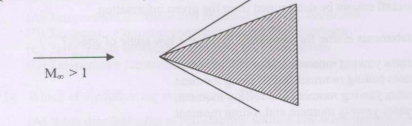
\includegraphics[width=0.5\linewidth]{figs/Screenshot from 2025-08-08 11-48-03.png}
    \caption{Caption}
    \label{fig:placeholder}
\end{figure}
An increase in free stream Mach number $M_\infty$ will cause the oblique shock wave to 
\begin{enumerate}
\begin{multicols}{2}
    \item move closer to the body 
    \item move away from the body 
    \item detach from the body 
    \item become a normal shock
    \end{multicols}
\end{enumerate}
 \hfill{GATE AE-2008}

    \quad

\item The geometrical features of a supercritical airfoil are  
\begin{enumerate}
\begin{multicols}{2}
    \item rounded leading edge, flat upper surface and high camber at the rear
    \item sharp leading edge, curved upper surface and high camber at the rear
    \item rounded leading edge, curved upper surface and no camber at the rear
    \item sharp leading edge, flat upper surface and no camber at the rear
    \end{multicols}
\end{enumerate}
 \hfill(GATE AE-2008)

    \quad

\item Which one of the following high lift device results in higher stalling angle? 
\begin{enumerate}
\begin{multicols}{2}
    \item split flap
    \item Fowler flap
    \item plain flap
    \item leading edge flap
    \end{multicols}
\end{enumerate}
 \hfill(GATE AE-2008)

    \quad

\item A turbofan engine has a bypass ratio of $5$ and a total mass flow rate of $120 \ \mathrm{kg/s}$. The mass flow rate through the bypass duct is
\begin{enumerate}
\begin{multicols}{2}
    \item $20 \ \mathrm{kg/s}$
    \item $100 \ \mathrm{kg/s}$
    \item $120 \ \mathrm{kg/s}$
    \item $600 \ \mathrm{kg/s}$
    \end{multicols}
\end{enumerate}
 \hfill(GATE AE-2008)

    \quad

\item A turbojet engine is operating with afterburner off. If the afterburner is switched on, then  
\begin{enumerate}
\begin{multicols}{2}
    \item both thrust and sfc decrease
    \item thrust increases and sfc decreases
    \item thrust decreases and sfc increases
    \item both thrust and sfc increase
    \end{multicols}
\end{enumerate}
 \hfill(GATE AE-2008)

    \quad

\item A centrifugal compressor operates with a tip blade speed of $340 \ \mathrm{m/s}$. The air leaves the impeller with a radial velocity of $88 \ \mathrm{m/s}$. If the slip factor is $0.85$, the relative velocity at the blade tip is  
\begin{enumerate}
\begin{multicols}{2}
    \item $101.7 \ \mathrm{m/s}$
    \item $120.3 \ \mathrm{m/s}$
    \item $132.6 \ \mathrm{m/s}$
    \item $135.8 \ \mathrm{m/s}$
    \end{multicols}
\end{enumerate}
 \hfill(GATE AE-2008)

    \quad

\item  An ideal ramjet engine is flying at a Mach number $M$. The exhaust gas static temperature at the outlet of the nozzle is $T_e$. The ambient static temperature is $T_a$. Gas constant $R$ and specific heat ratio $\gamma$ do not vary through the ramjet. Assuming that nozzle exhaust static pressure is equal to the ambient pressure and fuel air ratio $f \ll 1$, the thrust per unit mass flow rate is  
\begin{enumerate}
\begin{multicols}{2}
    \item $\sqrt{\gamma R T_a} \left[ \sqrt{\frac{T_e}{T_a}} - 1 \right]$
    \item $\sqrt{\gamma R T_e} \left[ \sqrt{\frac{T_e}{T_a}} - 1 \right]$
    \item $M \sqrt{\gamma R T_a} \left[ \sqrt{\frac{T_e}{T_a}} - 1 \right]$
    \item $M \sqrt{\gamma R T_e} \left[\sqrt{ \frac{T_e}{T_a}} - 1 \right]$
    \end{multicols}
\end{enumerate}
 \hfill(GATE AE-2008)

    \quad

\item A 50 percent degree of reaction axial flow turbine operates with a mean blade speed of $180 \ \mathrm{m/s}$. The flow leaves the stator and then enters the rotor at an angle of $60^\circ$ to the axial direction. The axial velocity is $150 \ \mathrm{m/s}$, and remains constant throughout the stage. The turbine power per unit mass flow is  
\begin{enumerate}
    \begin{multicols}{2}
    \item $29.76 \ \text{kJ/kg}$
    \item $41.12 \ \text{kJ/kg}$
    \item $58.33 \ \text{kJ/kg}$
    \item $61.13 \ \text{kJ/kg}$
    \end{multicols}
\end{enumerate}
\hfill(GATE AE-2008)

    \quad

\item The chamber stagnation temperature inside a rocket motor is $T_c$. Only a convergent nozzle is used, and the flow at the exit of this nozzle is choked. Assume that the nozzle exhaust static pressure is equal to ambient static pressure. Gas constant for exhaust gases is $R$ and ratio of specific heats is $\gamma$. The specific impulse of the rocket motor is  
\begin{enumerate}
\begin{multicols}{2}
    \item $\dfrac{2 \gamma R T_c}{\gamma - 1}$
    \item $\dfrac{\gamma R T_c}{\gamma - 1}$
    \item $\dfrac{\gamma R T_c}{\gamma + 1}$
    \item $\dfrac{2 \gamma R T_c}{\gamma + 1}$
    \end{multicols}
\end{enumerate}
\hfill(GATE AE-2008)

    \quad

\item  Air enters the combustor of a gas turbine engine at total temperature of $500 \ \mathrm{K}$ and leaves the combustor at total temperature of $1800 \ \mathrm{K}$. If $c_p$ remains constant at $1.005 \ \mathrm{kJ/(kg \cdot K)}$ and heating value of the fuel used is $44 \ \mathrm{MJ/kg}$, the fuel to air ratio is  
\begin{enumerate}
\begin{multicols}{4}
    \item $0.003$
    \item $0.012$
    \item $0.031$
    \item $0.074$
    \end{multicols}
\end{enumerate}
\hfill(GATE AE-2008)

    \quad

\item The initial temperature sensitivity of burn rate of a solid rocket motor propellant is positive. If the initial temperature increases then  
\begin{enumerate}
\begin{multicols}{2}
    \item thrust increases but burn time decreases
    \item thrust decreases and burn time decreases too
    \item thrust remains same but burn time increases
    \item thrust increases but burn time remains same
    \end{multicols}
\end{enumerate}
\hfill(GATE AE-2008)

    \quad

\item An aircraft is cruising at a Mach number of $0.8$ at an altitude where the ambient static pressure is $95 \ \mathrm{kPa}$. The diffuser exit total pressure is $140 \ \mathrm{kPa}$. Assuming there is no change in the specific heat at constant pressure across the diffuser, and ratio of specific heats is $1.4$, the adiabatic efficiency of the intake is  
\begin{enumerate}
\begin{multicols}{4}
    \item $0.988$
    \item $0.915$
    \item $0.722$
    \item $0.684$
    \end{multicols}
\end{enumerate}
\hfill(GATE AE-2008)

    \quad

\item A parallelogram shaped plate of dimensions 'a' and 'b' as shown in the figure, is subjected to a uniform loading of normal stresses $\sigma_1$ and $\sigma_2$. The plate is in equilibrium for 
\begin{figure}[H]
    \centering
    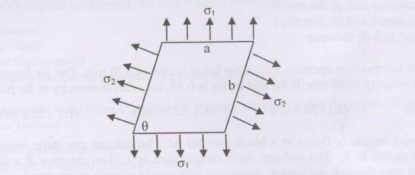
\includegraphics[width=0.5\linewidth]{figs/Screenshot from 2025-08-08 12-13-37.png}
    \caption{Caption}
    \label{fig:placeholder}
\end{figure}
\begin{enumerate}
\begin{multicols}{2}
    \item any value of $\sigma_1$ and $\sigma_2$
    \item $\sigma_2=\sigma_1 \cos\theta$
    \item $\sigma_1=\sigma_2 \cos\theta$
    \item $\sigma_2=\sigma_1$
    \end{multicols}
\end{enumerate}
\hfill(GATE AE-2008)

    \quad

\item A column of solid circular cross-section and length $L$ can have various end conditions. Choose the correct set that matches the end conditions (listed in Group I) with the corresponding effective length for buckling (listed in Group II).

\begin{center}
\begin{tabular}{|c|c|c|}
     \hline
     \textbf{Mineral} & \textbf{Modal abundance \brak{\%}} & \textbf{Partition coefficient}\\
     \hline
     Clinopyroxene & $45$ & $0.506$ \\
      \hline
      Orthopyroxene & $40$ & $0.42$ \\
      \hline
      Olivine & $10$ & $0.045$ \\
      \hline
      Plagioclase & $05$ & $0.019$ \\
      \hline
\end{tabular}
\end{center}

\quad

\begin{enumerate}
\begin{multicols}{2}

\item P-3, Q-1, R-2, S-4 
\item P-4, Q-1, R-2, S-3 
\item  P-2, Q-1, R-3, S-4 
\item P-3, Q-1, R-2, S-4
\end{multicols}
\end{enumerate}
\hfill(GATE AE-2008)

    \quad
    
\item A thin walled tube of circular cross-section with mean radius $r$ has a central web which divides it into two symmetric cells as shown. A torque $M$ is acting on the section. The shear flow $q$ in the central web is
\begin{figure}[H]
    \centering
    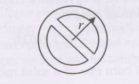
\includegraphics[width=0.5\linewidth]{figs/Screenshot from 2025-08-08 12-34-18.png}
    \caption{Caption}
    \label{fig:placeholder}
\end{figure}
\begin{enumerate}
\begin{multicols}{4}
    \item $q=M/2\pi r^2$
     \item $q=0$
      \item $q=M/4\pi r^2$
       \item $q=M/\pi r^2$
       \end{multicols}
\end{enumerate}
\hfill(GATE AE-2008)

\quad 

\item  A concentraion bending moment M is acting at mid-span of a beam as shown. The shear force diagram for the beam is:
\begin{figure}[H]
    \centering
    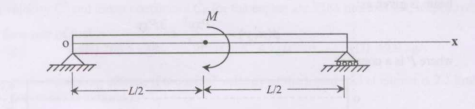
\includegraphics[width=0.5\linewidth]{figs/Screenshot from 2025-08-08 12-52-57.png}
    \caption{Caption}
    \label{fig:placeholder}
\end{figure}
\begin{enumerate}
    \item 
    \begin{figure}[H]
        \centering
        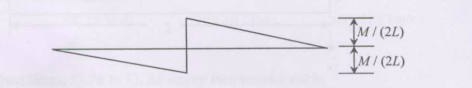
\includegraphics[width=0.5\linewidth]{figs/Screenshot from 2025-08-08 12-59-04.png}
        \caption{Caption}
    \label{fig:placeholder}
    \end{figure} 
    
    \item 
    \begin{figure}[H]
        \centering
        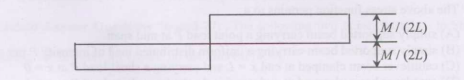
\includegraphics[width=0.5\linewidth]{figs/Screenshot from 2025-08-08 14-37-14.png}
        \caption{Caption}
    \label{fig:placeholder}
        \end{figure} 

        \item 
        \begin{figure}[H]
            \centering
            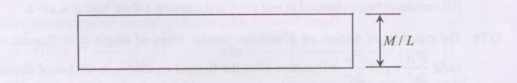
\includegraphics[width=0.5\linewidth]{figs/Screenshot from 2025-08-09 16-17-42.png}
            \caption{Caption}
    \label{fig:placeholder}
        \end{figure}

        \item 
        \begin{figure}[H]
            \centering
            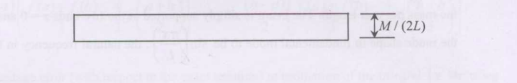
\includegraphics[width=0.5\linewidth]{figs/Screenshot from 2025-08-09 16-19-48.png}
            \caption{Caption}
    \label{fig:placeholder}
        \end{figure}
        
\end{enumerate}
\hfill(GATE AE-2008)

\quad

\item  An idealized thin-walled cross-section of a beam and the respective areas of the booms are as shown. A bending moment M, is acting on the cross-section. The ratio of the magnitude of normal stress in the top booms to that of the bottom boom is
\begin{figure}[H]
    \centering
    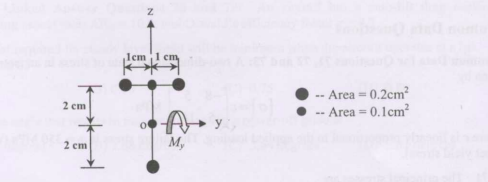
\includegraphics[width=0.5\linewidth]{figs/Screenshot from 2025-08-08 14-45-55.png}
    \caption{Caption}
    \label{fig:placeholder}
\end{figure}
\begin{enumerate}
\begin{multicols}{4}
    \item 5/11
    \item 2/5
    \item 1
    \item 5/2
    \end{multicols}
\end{enumerate}
\hfill(GATE AE-2008)

\quad

\item  An engineer is asked to test a system which can be idealized as SDOF (single degree of freedom) with viscous damping. A frequency response test was conducted and it is found that the quality factor Q is equal to 10. What will be the logarithmic decrement if a free vibration test is performed?
\begin{enumerate}
\begin{multicols}{4}
    \item $\pi/40$
     \item $\pi/20$
     \item $\pi/10$
      \item $\pi/5$
      \end{multicols}
\end{enumerate}
\hfill{GATE AE-2008}

\quad

\item A beam occupies a region 
$
0 \leq x \leq L, \quad -c \leq y \leq c, \quad -0.5 \leq z \leq 0.5
$
as shown below. The beam can be considered to be in plane stress condition in the $x\text{-}y$ plane.  
Airy's stress function for the beam is given as:
$
\phi(x,y) = \frac{Pxy^{3}}{4c^{3}} + \frac{3Pxy}{4c}
$
where $P$ is a constant.
\begin{figure}[H]
    \centering
    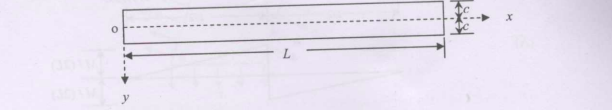
\includegraphics[width=0.5\linewidth]{figs/Screenshot from 2025-08-08 14-58-40.png}
    \caption{Caption}
    \label{fig:placeholder}
\end{figure}
The above stress function pertains to a 
\begin{enumerate}
\begin{multicols}{2}
\item simply supported beam carrying a point load P at mid span
\item simply supported beam carrying a uniform distributed load of intensity P per unit length
\item cantilever beam clamped at end x = L and carrying a shear load P at x = 0
\item cantilever beam clamped at end x = 0 and carrying a shear load P at 
\end{multicols}
\end{enumerate}
\hfill(GATE AE 2008)

\quad 

\item  The equation of motion of a uniform slender beam of length \( L \) in flexural vibration is given as
$
EI \frac{\partial^4 w}{\partial x^4} + \rho A \frac{\partial^2 w}{\partial t^2} = 0
$
where $EI$ is the flexural rigidity, $w$ is the lateral displacement and $ \rho A $ is the mass per unit length.  
The beam is simply supported at the two ends $x = 0 $and $x = L $.  
Assuming the mode shape in fundamental mode to be $ \sin\left( \frac{\pi x}{L} \right) $,  
the natural frequency in fundamental mode is:

\begin{enumerate}
\begin{multicols}{2}
\item $ 0.5 \sqrt{\frac{EI}{\rho A L^4}} \, \pi^2 $
\item $sqrt{\frac{EI}{\rho A L^4}} \, \pi^2 $
\item $ 2 \sqrt{\frac{EI}{\rho A L^4}} \, \pi^2$ 
\item $ 4 \sqrt{\frac{EI}{\rho A L^4}} \, \pi^2$
\end{multicols}
\end{enumerate}
\hfill(GATE AE 2008)

\quad 

\textbf{Common Data Questions}  

\quad

\textbf{Common Data for Questions 71, 72 and 73:}  
A two-dimensional state of stress in an isotropic material is given by:
$
[\sigma] = c 
\myvec{
-8 & 5 \\
5 & 16
} \; \text{MPa}
$
where $c$ is linearly proportional to the applied loading.  
The failure stress is $ \sigma_f = 350 \, \text{MPa}$ (which is 0.2\% offset yield stress).

\item The principal stresses are:  

\begin{enumerate}
\begin{multicols}{2}
    \item $\sigma_1=17cMPa$, $\sigma_2=-9cMPa$
    \item $\sigma_1=9cMPa$, $\sigma_2=17cMPa$
    \item $\sigma_1=-17cMPa$, $\sigma_2=-9cMPa$
    \item $\sigma_1=17cMPa$, $\sigma_2=9cMPa$
    \end{multicols}
\end{enumerate}
\hfill(GATE AE 2008)

\quad 

\item The maximum shear stress is: 
\begin{enumerate}
\begin{multicols}{2}
    \item $\tau_{max}=7cMPa$
    \item $\tau_{max}=10cMPa$
    \item $\tau_{max}=13cMPa$
    \item $\tau_{max}=15cMPa$
    \end{multicols}
\end{enumerate}
\hfill(GATE AE 2008)

\quad 

\item The maximum value of $c $ for safe loading of the structure, based on von-Mises failure criterion is:  
\begin{enumerate}
\begin{multicols}{4}
    \item 10.2
    \item 15.3
    \item 25.4
    \item 31.8
    \end{multicols}
\end{enumerate}
\hfill(GATE AE 2008)

\quad 

\textbf{Common Data for Questions 74 and 75:}  
A liquid rocket engine with oxidizer to fuel ratio of 5:1 produces a thrust of $ 1 \, \text{MN} $.  
The initial mass of the rocket engine is $ 100{,}000 \, \text{kg} $ and its mass at burn out is $10{,}000 \, \text{kg} $.  
The characteristic velocity $C^* $ and thrust coefficient $C_F $ for the engine are 2386 \text{m/s}  and 1.4 , respectively.

\item The mass flow rate of fuel is:  
\begin{enumerate}
   \begin{multicols}{4}
\item 300.3 kg/s
\item 269.5 kg/s
\item 87.4 kg/s 
\item 49.9 kg/s
\end{multicols}
\end{enumerate}
\hfill(GATE AE 2008)

\quad 

\item Neglecting gravity and drag effects, if the initial velocity of the liquid rocket engine is $2.5 \ \text{km/s}$, the velocity of the rocket at burnout is:  

\begin{enumerate}
\begin{multicols}{2}
\item $1.2 \ \text{km/s}$
\item $2.5 \ \text{km/s}$
\item $10.2 \ \text{km/s}$
\item $11.8 \ \text{km/s}$
\end{multicols}
\end{enumerate}
\hfill(GATE AE 2008)

\quad 

\textbf{Statement for Linked Answer Questions 76 and 77:} 
The following two questions relate to Simpson's rule for approximating the integral  
$\int_a^b f(x) \, dx$ on the interval $[a, b]$.

\item Which of the following gives the correct formula for Simpson's rule? 

\begin{enumerate}
\begin{multicols}{2}
\item $\dfrac{(b-a)}{2} \left[ f(b) + f\left( \dfrac{a+b}{2} \right) \right]$
\item $\dfrac{(b-a)}{2} \left[ f(a) + f(b) + f\left( \dfrac{a+b}{2} \right) \right]$
\item $\dfrac{(b-a)}{2} \left[ \dfrac{f(a) + f(b)}{3} + \dfrac{4}{3} f\left( \dfrac{a+b}{2} \right) \right]$
\item $\dfrac{(b-a)}{2} \left[ \dfrac{f(a) + f(b)}{3} + \dfrac{4}{3} f\left( \dfrac{a+b}{3} \right) \right]$
\end{multicols}
\end{enumerate}
\hfill(GATE AE 2008)

\quad 

\item The percentage error (with respect to the exact solution) in estimation of the integral  
$\int_{0}^{1} x^3 \, dx$ using Simpson's rule is:  

\begin{enumerate}
\begin{multicols}{4}
\item $5.3$
\item $3.5$
\item $2.8$
\item $0$
\end{multicols}
\end{enumerate}
\hfill(GATE AE 2008)

\quad 

\textbf{Statement for Linked Answer Questions 78 and 79:}  
An aircraft has a zero-lift drag coefficient $C_{D_0} = 0.0223$, wing aspect ratio $AR_w = 10.0$, and Oswald's efficiency factor $e = 0.7$.

\item The thrust required for steady level flight will be minimum when the aircraft operates at a lift coefficient of:  

\begin{enumerate}
\begin{multicols}{4}
\item $0.65$
\item $0.70$
\item $0.75$
\item $0.80$
\end{multicols}
\end{enumerate}
\hfill(GATE AE-2008)

\quad 

\item The glide angle that results in maximum range in a power-off glide is:  

\begin{enumerate}
\begin{multicols}{4}
\item $1.82^\circ$
\item $2.68^\circ$
\item $3.64^\circ$
\item $5.01^\circ$
\end{multicols}
\end{enumerate}
\hfill(GATE AE 2008)

\quad 

\textbf{Statement for Linked Answer Questions 80 and 81:}  
Consider an untwisted wing of elliptical planform in inviscid incompressible irrotational flow at an angle of attack of $4^\circ$.  
The wing aspect ratio is $7$ and the zero lift angle of attack is $-2^\circ$.\\

\item The wing lift coefficient $C_L$ is:  

\begin{enumerate}
\begin{multicols}{4}
\item $0.66$
\item $0.51$
\item $0.44$
\item $0.34$
\end{multicols}
\end{enumerate}
\hfill(GATE AE 2008)

\quad 

\item The induced drag coefficient of the wing $C_{D_i}$ is:  

\begin{enumerate}
\begin{multicols}{4}
\item $0.0053$
\item $0.0087$
\item $0.0118$
\item $0.0197$
\end{multicols}
\end{enumerate}
\hfill(GATE AE 2008)

\quad 

\textbf{Statement for Linked Answer Questions 82 and 83:}  
A multi-stage axial flow compressor operating at an adiabatic efficiency of $0.9$ develops a total pressure ratio of $11$.  
The total temperature at inlet to the compressor is $335 \ \text{K}$ and the stagnation enthalpy rise across each stage is $37 \ \text{kJ/kg}$.  
Ratio of specific heats is $1.4$ and specific heat at constant pressure is $1.005 \ \text{kJ/kg.K}$.

\item The total temperature rise across the compressor is:  

\begin{enumerate}
\begin{multicols}{4}
\item $310.1 \ \text{K}$
\item $366.3 \ \text{K}$
\item $392.1 \ \text{K}$
\item $405.4 \ \text{K}$
\end{multicols}
\end{enumerate}
\hfill(GATE AE 2008)

\quad

\item The total number of stages required are:  

\begin{enumerate}
\begin{multicols}{4}
\item $9$
\item $10$
\item $11$
\item $12$
\end{multicols}
\end{enumerate} 
\hfill(GATE AE 2008)

\quad

\textbf{Statement for Linked Answer Questions 84 and 85:}  
An idealized thin walled two cell symmetric box beam is as shown.  
The shear flows in the walls are due to the applied shear forces $V_y = 480 \ \text{N}$, $V_z = 300 \ \text{N}$, and a torque $M$, all acting at the shear center.

\begin{figure}[H]
    \centering
    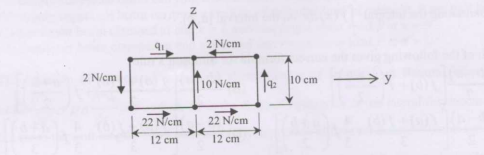
\includegraphics[width=0.5\linewidth]{figs/pic9.png}
    \caption{Caption}
    \label{fig:placeholder}
\end{figure}

\item \quad The shear flows $q_1$ and $q_2$ are:  

\begin{enumerate}
\begin{multicols}{2}
\item $q_1 = -2 \ \text{N/cm}$, \quad $q_2 = +22 \ \text{N/cm}$
\item $q_1 = +2 \ \text{N/cm}$, \quad $q_2 = +22 \ \text{N/cm}$
\item $q_1 = +2 \ \text{N/cm}$, \quad $q_2 = -22 \ \text{N/cm}$
\item $q_1 = -2 \ \text{N/cm}$, \quad $q_2 = -22 \ \text{N/cm}$
\end{multicols}
\end{enumerate} 
\hfill(GATE AE 2008)

\quad

\item The torque $M$ is:  

\begin{enumerate}
\begin{multicols}{2}
\item $3360 \ \text{N.cm}$
\item $5760 \ \text{N.cm}$
\item $6960 \ \text{N.cm}$
\item $8160 \ \text{N.cm}$
\end{multicols}
\end{enumerate} 
\hfill(GATE AE 2008)

\quad
\end{enumerate}
\end{document}
